\section{Aggregating Induced Views}
\label{sec:aggregation}
In the previous sections, we introduced four strategies to identify the accepted answer to a question. Each strategy induces a graph or relational view between $(q,a)$ tuples.
Each relational view is expected to capture semantically diverse neighborhoods of vertices. The convolution operator aggregates the neighborhood information under each view. The key question that follows is, \emph{how do we combine these diverse views in a unified learning framework?} Past work has considered multiple solutions:
\begin{itemize}
  \label{item:aggregator}
\item \textbf{Neighborhood Aggregation}: In this approach, they represent vertices by aggregating feature representations of it's neighbors across all views \cite{graphsage, relationalGCN}. Specifically, the final adjacency matrix is the sum of all the individual adjacency matrices of each view, i.e., $A = \sum_{S_i \in \mathbf{S}} A_i$. They, then, apply Graph Convolution Network to this updated Adjacency matrix.
\item \textbf{Stacking}: Multiple convolution layers stacked end-to-end (each potentially handling a different view) \cite{Stacking}. Specifically, they stacks all GCNs belonging to a view such that output of a lower GCN is fed as an input to the GCN directly above it. Thus, output from the last layer of GCN for view $i$, $Z_i^K$ s.t. $  S_i \in \textbf{S}$ will act as input features, $Z_j^0$ for some other view $j$ s.t. $S_j \in \{\textbf{S}-S_i \}$ if view $j$ is directly above the view $i$. In our experiments, we obtain the best performance by using the following order: Contrastive, Similarity by Contrast followed by Reflexive.
\item \textbf{Fusion}: Follows a multi-modal fusion approach~\cite{Fusion18}, where views are considered distinct data modalities. It treats each GCN as a separate model and appends the output from the final layer of each GCN i.e. $Z_i^K; \forall S_i \in \textbf{S}$ to the input of all the other GCN's, i.e. $Z_j^0 \forall S_j \in \textbf{S}-S_i$ along with the original features. Thus, the input of each GCN is linear in $\vert \textbf{S} \vert$.
\item \textbf{Shared Latent Structure}: Attempts to transfer knowledge across relational views (modalities) with constraints on the representations (e.g. \cite{DualGCN} aligns embeddings across views).
\end{itemize}

Ensemble methods introduced in \cite{relationalGCN} work on multi-relational edges in knowledge graphs. None of these approaches are directly suitable for our induced relationships. Our relational views utilize different label assignment semantics (label sharing within a clique vs. determine label based on contrast within a clique). In our label contrast semantics, we must achieve feature discrimination and label inversion between contrasting vertices, as opposed to label homogeneity and feature sharing in the label sharing case. Thus, aggregating relationships by pooling, concatenation, or addition of vertex representations fail to capture semantic heterogeneity of the induced views.
Further, data induced relations are uncurated and inherently noisy. Directly aggregating the learned representations via Stacking or Fusion can lead to noise propagation. We also expect views of the same relation type to be correlated.

\begin{figure}[tbh]
    \centering
    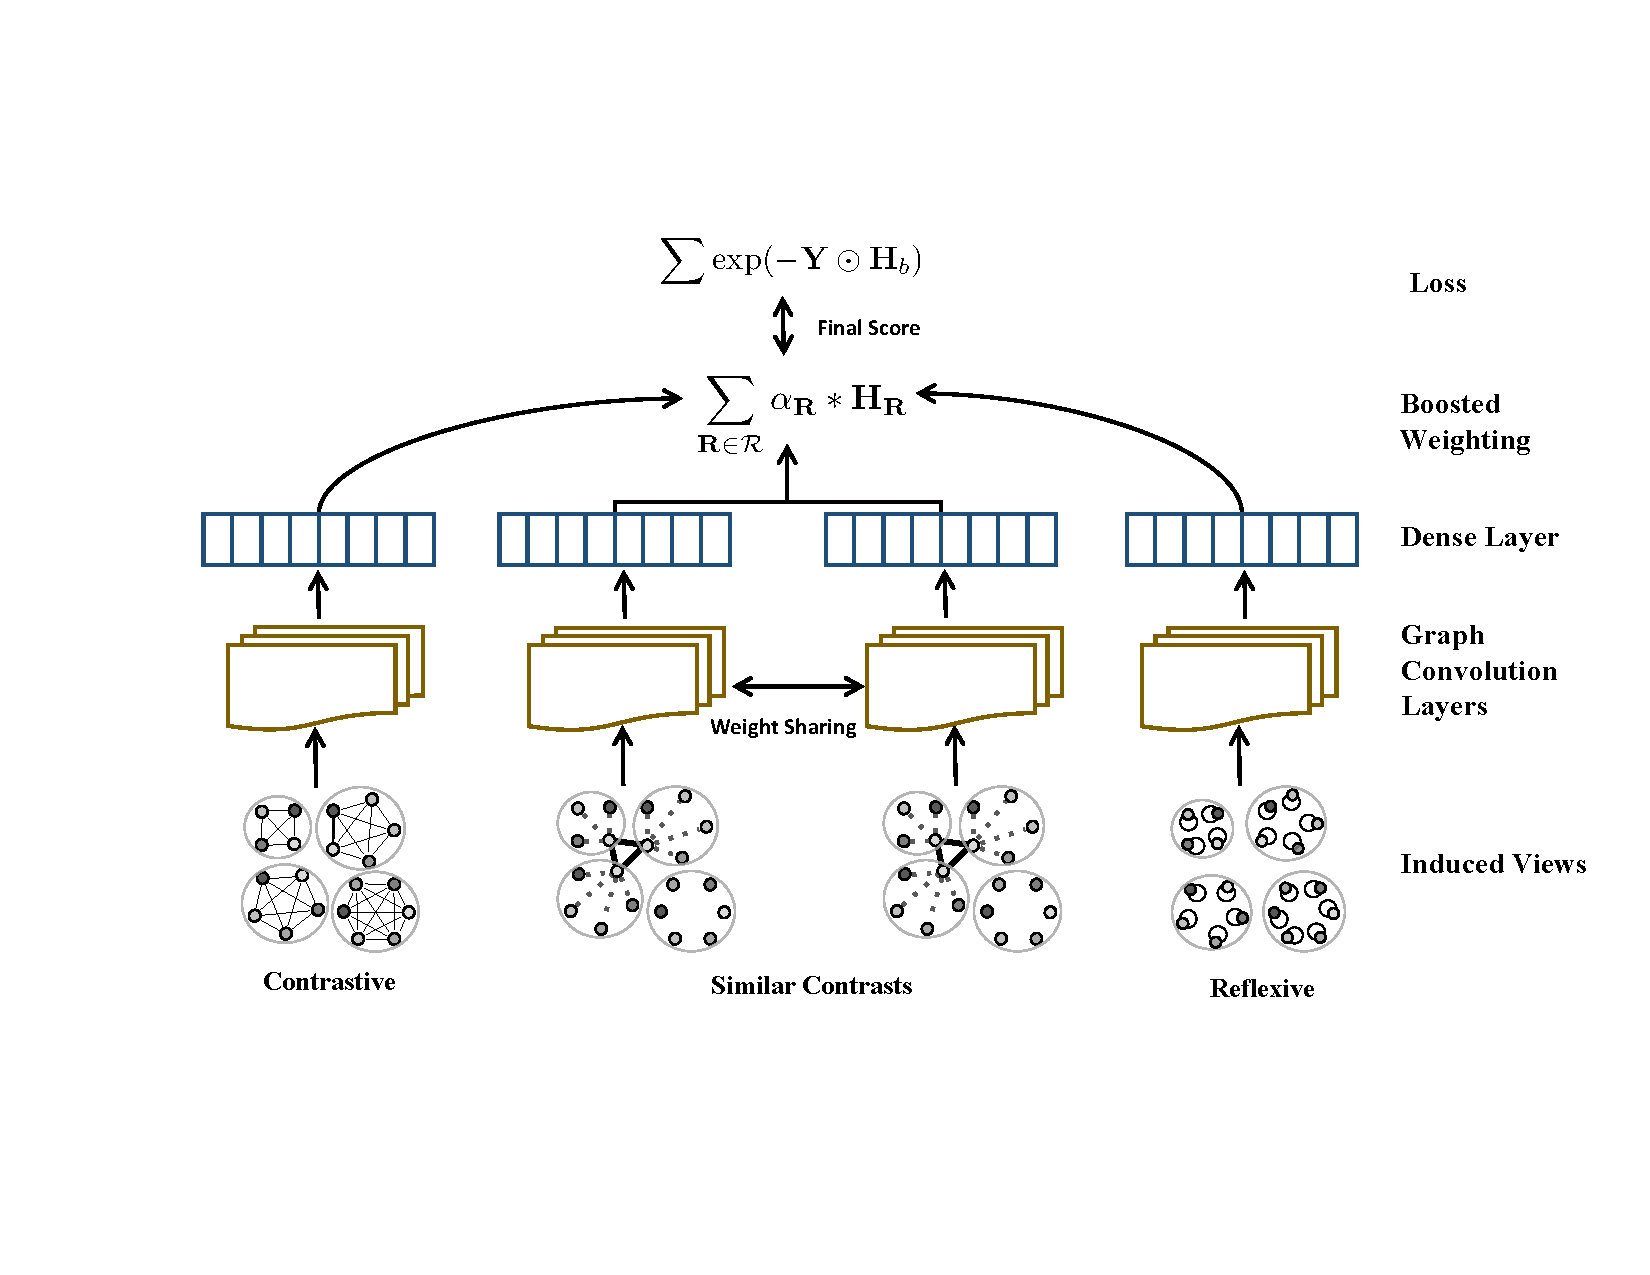
\includegraphics[scale=0.67]{figures/Architecture_new.pdf}
    \caption{\label{fig:adaboost} Schematic diagram of our proposed IR-GCN model.}
\end{figure}

We thus propose the following approach to aggregate information across relation types and between views of a relation type.

\noindent
\textbf{Cross-relation Aggregation}: We expect distinct relation types to perform well on different subsets of the set of $(q,a)$ tuples. We empirically verify this with the Jaccard overlap between the set of misclassified vertices under each relational view of a relation type on our dataset. Given $\mathbf{M}_A$ and $\mathbf{M}_B$, the sets of $(q,a)$ tuples misclassified by GCNs $A$ and $B$ respectively, the jaccard overlap is,
\begin{equation}
 \mathcal{J}_{A,B} = \frac{\mathbf{M}_A \cap \mathbf{M}_B}{\mathbf{M}_A \cup \mathbf{M}_B}
\end{equation}
The $\mathcal{J}_{A,B}$ values are as follows for the relational pairings: (Contrastive, TrueSkill Similarity) = 0.42, (Contrastive, Reflexive) = 0.44 and (Reflexive, TrueSkill Similarity) = 0.48. Relatively low values of the overlap metric indicate uncorrelated errors across the relations.

Gradient boosting techniques are known to improve performance when individual classifiers, including neural networks \cite{ncboost}, are diverse yet accurate. A natural solution then is to apply boosting to the set of relation types and bridge the weaknesses of each learner. We employ Adaboost \cite{adaboost} to combine relation level scores, $\mathbf{H}_{\mathbf{R}}$ (~\cref{eq:score}) in a weighted manner to compute the final boosted score, $\mathbf{H}_b \in \mathbb{R}^{N \times 1}$ representing all relation types (Line 12, ~\cref{alg:inference}). $\mathbf{Y} \in \mathbb{R}^{N X 1}$ denotes the acceptance label of all tuples. Note that an entry in $(\mathbf{Y} \odot \mathbf{H_{\mathbf{R}}}) > 0 $ when the accepted label of the corresponding $(q,a)$ tuple and sign of the prediction score, $sign(\mathbf{H_{\mathbf{R}}})$, of relation type $\mathbf{R}$ match and $< 0$ otherwise. Thus, the weights $\alpha_\mathbf{R}$ adapt to the fraction of correctly classified tuples to the misclassified tuples by the relation $\mathbf{R}$ (Line 9, ~\cref{alg:inference}).
The precise score computation is described in ~\cref{alg:inference}. We use the polarity of each entry in the boosted score, $sign(\mathbf{H}_b) \in \{-1,1 \}$, to predict the class label of the corresponding $(q,a)$ tuple. The final score is also used to create a ranked list among all the candidate answers, $a \in \mathcal{A}(q)$ for each question, $q \in \mathcal{Q}$. $L_{(q,a)}$ represents the position of candidate answer $a$ in the ranked list for question $q$.

\noindent
\textbf{Intra-relation Aggregation}: Gradient boosting methods can effectively aggregate relation level representations, but are not optimal within a relationship type (since it cannot capture shared commonalities between different views of a relation type). For instance, we should facilitate information sharing between the TrueSkill similarity and Arrival similarity views. Thus, if an answer is authored by a user with a higher skill rating and answered significantly earlier than other answers, its probability to be accepted should be mutually enhanced by both signals. Empirically, we also found True Skill and Arrival Similarity GCNs to commit similar mistakes ($\mathcal{J}_{TS,AS}$ = 0.66). Thus, intra-relation learning (within a single relation type like Similar Contrast) can benefit from sharing the structure of their latent spaces i.e., weight parameters of GCN.

\begin{algorithm}[tbh]
\caption{IR-GCN Boosted Score Computation}\label{alg:inference}
\begin{algorithmic}[1]
\Function{Forward}{$\mathbf{X}, \mathbf{Y}, \{A_i\}_{S_i \in \mathbf{S}}$}
  \State $\mathbf{H}_{b} \gets \mathbf{0} $
    \For{$\mathbf{R} \in \mathcal{R}$}
    \State $\{ \mathbf{Z}_i^K \}_{S_i \in \mathbf{R}} \gets Conv(\mathbf{X}, \{ A_i \}_{S_i \in \mathbf{R}})$
    \State \Comment{Equation  \ref{eq:contrast}, \ref{eq:similar}, \ref{eq:reflexive}}
    \State $\mathbf{H}_\mathbf{R} =\sum_{{S_i} \in \mathbf{R}} \mathbf{Z}_i^{K} \times \widetilde{\mathbf{W}}_i$ \Comment{Equation \ref{eq:score}}
    %\State $h_s = merge(h_{as}, h_{ts})$ \Comment{Equation \ref{eq:merge}}
    \State $ \mathbf{e}_{\mathbf{R}} \gets \exp({-\mathbf{Y} \odot \mathbf{H}_{b}})$
    \State \Comment{ $\odot \rightarrow \textit{Hadamard Product}$}
  \State $\alpha_\mathbf{R} \gets \dfrac{1}{2} \ln{\dfrac{\sum \mathbf{e}_{\mathbf{R}} \odot \mathbbm{1}\left((\mathbf{Y} \odot \mathbf{H}_{\mathbf{R}}\right) > 0)}{\sum \mathbf{e}_{\mathbf{R}} \odot \mathbbm{1}\left((\mathbf{Y} \odot \mathbf{H}_{\mathbf{R}}) < 0 \right) }}$
    \State \Comment{$\sum \rightarrow \textit{reduce-sum}$}
      \State \Comment{$\mathbbm{1}(.) \rightarrow \textit{element-wise Indicator function}$}
  \State    $\mathbf{H}_{b} \gets \mathbf{H}_{b} + \alpha_\mathbf{R} * \mathbf{H}_{\mathbf{R}}$ \Comment{Update boosted GCN}
    \EndFor
    \State \Return $\mathbf{H}_{b}$, $ \{ \mathbf{H}_{R} \}_{\mathbf{R} \in \mathcal{R}}$, $\{ \mathbf{Z}_{i}^{K} \}_{S_i \in \mathbf{S}}$
    \State \Comment{Boosted scores, Relation level scores,}
    \State \Comment{Each GCN vertex representations}
\EndFunction
\end{algorithmic}
\end{algorithm}

\noindent
\emph{Weight Sharing:} For multiple views representing a relation type (e.g., TrueSkill and Arrival Similarity), we train a separate GCN for each view but share the layer-wise linear-transforms $\mathbf{W}_i^{k}$ to capture similarities in the learned latent spaces.
Weight sharing is motivated by a similar idea explored to capture local and global views in \cite{DualGCN}. Although sharing the same weight parameters, each GCN can still learn distinct vertex representations as each view convolves over a different neighborhood and employ random dropout during training.
We thus propose to use an alignment loss term to minimize prediction difference between views of a single relation type\cite{reg}. The loss attempts to align the learned vertex representations at the \emph{last layer} $K$ (the loss term aligns pairs of final vertex representations, $\lvert\lvert \mathbf{Z}_i^{K} - \mathbf{Z}_{i'}^{K} \lvert\lvert \texttt{  }\forall\texttt{ } S_i, S_i' \in \mathbf{R}$). In principle, multiple GCNs augment performance of the relation type by sharing prior knowledge through multiple Adjacency matrices ($\mathbf{A}_i \texttt{  }\forall\texttt{ } S_i \in \mathbf{R}$).

\begin{algorithm}[!h]
\caption{IR-GCN Training}\label{alg:training}
\begin{algorithmic}[1]
\Require{Input Feature Matrix $X$, Acceptance labels for each tuple, $\mathbf{Y}$, Adjacency matrix of each view $\{A_i\}_{S_i \in \mathbf{S}}$ }
\Ensure{Trained Model i.e. Weight parameters $W_{i}^{1} \ldots W_{i}^{k}, S_i \in \mathbf{S}, \forall k \in [1, K]$ and transform parameters $\widetilde{W}_i$, $S_i \in \mathbf{S}$ }
\For{$t \gets 1$ to $\textit{num-epochs}$}
    \State $\mathbf{H}_b, \{ \mathbf{H}_{R} \}_{\mathbf{R} \in \mathcal{R}}, \{ \mathbf{Z}^{K}_{i} \}_{S_i \in \mathbf{S}}$$\gets \textsc{Forward}(X, Y, \{ A_i \}_{S_i \in \mathbf{S}})$
    \State \Comment{\Cref{alg:inference}}
    \For{ $\mathbf{R} \in \mathcal{R}$}

        \State $\mathcal L_b \gets \sum \exp({-\mathbf{Y} \odot \mathbf{H}_b}) + \gamma_1 \mathcal L_1(.) + \gamma_2 \mathcal L_2(.)$
    \State \Comment{$\sum \rightarrow \textit{reduce-sum}$}
  \State \Comment{$\odot \rightarrow \textit{Hadamard Product}$}
        \State $\mathcal L_{\mathbf{R}} \gets 0$
        \For{ $S_i \in \mathbf{R}$}
        \State $\mathcal L_{i} \gets \sum \exp({-\mathbf{Y} \odot \mathbf{H}_\mathbf{R}})$
    \State $\mathcal L_{\mathbf{R}} \gets \mathcal L_{\mathbf{R}} + \mathcal L_{i} + \frac{1}{2}\sum_{S_i' \neq S_i}\lvert\lvert \mathbf{Z}_{i}^K - \mathbf{Z}_{i'}^K \lvert\lvert $
    \EndFor
    \State $\mathcal L_b \gets \mathcal L_b + \lambda(t) \mathcal L_{\mathbf{R}}$
    \State    $W_i^{k} \gets  W_i^{k} + \eta_{\textsc{adam}} \frac{\partial \mathcal L_b}{\partial W_i^{k}} $ \Comment{$\forall k \in [1, K], \forall S_i \in \mathbf{R}$}
     \State    $\widetilde{W}_i \gets  \widetilde{W}_i +  \eta_{\textsc{adam}} \frac{\partial \mathcal L_b}{\partial \widetilde{W}_i}$ \Comment{$\forall S_i \in \mathbf{S}$}
    \EndFor
\EndFor
\end{algorithmic}
\end{algorithm}

\noindent
\textbf{Training Algorithm}: Algorithm \ref{alg:training} describes the training algorithm for our IR-GCN model. For each epoch, we first compute the aggregated prediction score $\mathbf{H}_{b}$ of our boosted model as described in \cref{alg:inference}. We use a supervised exponential loss $\mathcal{L}_b$ for training with elastic-net regularization (L1 loss - $\mathcal L_1(.)$ and L2 loss - $\mathcal L_2(.) $) on the graph convolutional weight matrices $\mathbf{W}_{\mathbf{i}}^{k} \texttt{  }\forall\texttt{ } S_i \in \mathbf{S}$ for each view. Note that we employ weight sharing between all views of the same relation type so that only one set of weight matrices is learned per relation. %The views in our training are Contrast (c), TrueSkill (ts), Arrival Similarity (as) and Reflexive view (r).

The exponential loss, $\mathcal{L}_{\mathbf{R}}$, for each relation type is added alternatingly to the boosted loss.
We apply an \emph{exponential annealing schedule}, $\lambda(t)$, i.e. a function of the training epochs ($t$), to the loss function of each relation. As training progresses and the boosted model learns to optimally distribute vertices among the relations, increase in $\lambda(t)$ ensures more emphasis is provided to the individual convolutional networks of each relation. Figure \ref{fig:adaboost} illustrates the overall architecture of our IR-GCN model.
